\renewcommand{\baselinestretch}{1.5}

\chapter{Workplan}

This chapter organizes the work needed to carry out the experimental design of Chapter~IV. The work is planned by calendar month (Figure~\ref{fig:gantt}): the corrections of this proposal take place from November 2026 to January 2027, the research phase starts in February 2027, and the delivery of the thesis is expected about October 2027. The periods are estimates.

\section{Tasks}

\subsection{Proposal and Literature}

\begin{itemize}
  \item Finish the research proposal: related work, the state of the art, and the corrections requested by the advisor.
  \item Keep the literature search up to date with the strings and sources of Chapter~II, and read in full the works that are closest to the hypothesis.
\end{itemize}

\subsection{Code and Infrastructure}

\begin{itemize}
  \item Add a switch that turns off the variational output layer of the decoder, so that factor E can be tested.
  \item Make every replicate use its own seed for the VAE and for the generator, and record the seeds.
  \item Integrate masking and image selection in the training of the VAE as factors that can be switched on and off from the configuration.
  \item Write the evaluation scripts (FID, KID, PSNR, SSIM, and the FID of the reconstructions) so that every run is evaluated in the same way.
  \item Sample the generated images in batches, so that the number of images chosen in Stage~0 is affordable.
  \item Generate the fractional design, check its aliasing, and randomize the order of the runs; write the analysis script in R.
  \item Define the workflow of the cluster: at most four jobs at a time, evaluation after each run, and archiving or deletion of checkpoints to respect the storage quota.
\end{itemize}

\subsection{Stage 0: Noise and Convergence}

Train five replicates of the base cell, check that the VAE converges with the fixed number of epochs, estimate the standard deviation of the FID between independent runs, set the margin of the equivalence tests, and choose the number of generated images $N$ by comparing the sampling noise of the FID with the variation between runs (Chapter~IV).

\subsection{Stage 1: Screening}

Run the $2^{6-2}$ design with DDPM and three replicates per cell (48 runs; the period reserved for this stage leaves room for up to five replicates), evaluate every run, and analyze the results with the analysis of variance, the equivalence tests, and the correlation between reconstruction and generation.

\subsection{Stage 2: Refinement}

Choose the factors that showed an effect and study them with a full factorial design and more levels, resolving the interactions that were aliased in Stage 1.

\subsection{Stage 3: Confirmation with Flow Matching}

Repeat the factors that mattered with Flow Matching (FM) in a small full factorial design, to check that the effect does not depend on the generator.

\subsection{Optional Work}

\begin{itemize}
  \item If time permits, prototype a pretrained self-supervised encoder (DINO) as an alternative latent space (objective 5).
  \item If an opportunity arises, a month, flexible within the schedule, could be used to apply the findings to a second crop with UAV imagery, for example during a research exchange in Osnabr\"uck; this is not part of the objectives, and the runs of the cluster can continue during it.
\end{itemize}

\subsection{Paper and Thesis}

Write a paper with the results of the study (objective 6) and write the thesis. The drafting starts in February with the introduction, the related work, and the method, which this proposal already contains, and the results are added as each stage ends.

\section{Schedule}

Table~\ref{tab:schedule} shows the phases with their period and the computing time they need. The computing times come from the budget of Chapter~IV (about 26 hours per generator and about 14 hours per VAE trained from scratch, with four jobs in parallel); the durations include time for the queue of the cluster and for runs that must be repeated.

\begin{table}[H]
\centering
\small
\begin{tabular}{p{0.30\textwidth}p{0.17\textwidth}p{0.24\textwidth}p{0.21\textwidth}}
\hline
\textbf{Phase} & \textbf{Period (2027)} & \textbf{Computing} & \textbf{Output} \\
\hline
Proposal and corrections & Nov 2026 to Jan & -- & Approved proposal \\
Code and infrastructure & Feb to Mar & -- & Switch, seeds, batched sampling, scripts, design \\
Stage 0: noise and convergence & Apr & about 200 GPU hours (4 days), plus the sampling for $N$ & Standard deviation, epochs, margin, $N$ \\
Stage 1: screening & May to Jun & about 1\,900 GPU hours (20 days); room for five replicates & 48 evaluated runs \\
Analysis of Stage 1 & Jul & -- & Factors that matter \\
Stage 2: refinement & Jul to Aug & about 700 GPU hours (8 days)\textsuperscript{a} & Effects and interactions \\
Stage 3: confirmation & Aug to Sep & about 420 GPU hours (5 days) & Check with FM \\
Final analysis and thesis & Sep to Oct & -- & Thesis \\
Paper and thesis drafting & Feb to Sep (parallel) & -- & Paper draft \\
Optional: DINO extension & Jul to Sep & -- & Prototype \\
Optional: stay in Osnabr\"uck & one month, Apr to Sep & -- & Cross-crop check \\
\hline
\end{tabular}
\caption{Phases of the work. \textsuperscript{a}Estimate that depends on the factors selected in Stage 1. The drafting of the paper starts in February and the results are added as they appear; the stay in Osnabr\"uck is a flexible month.}
\label{tab:schedule}
\end{table}

\begin{figure}[H]
\centering
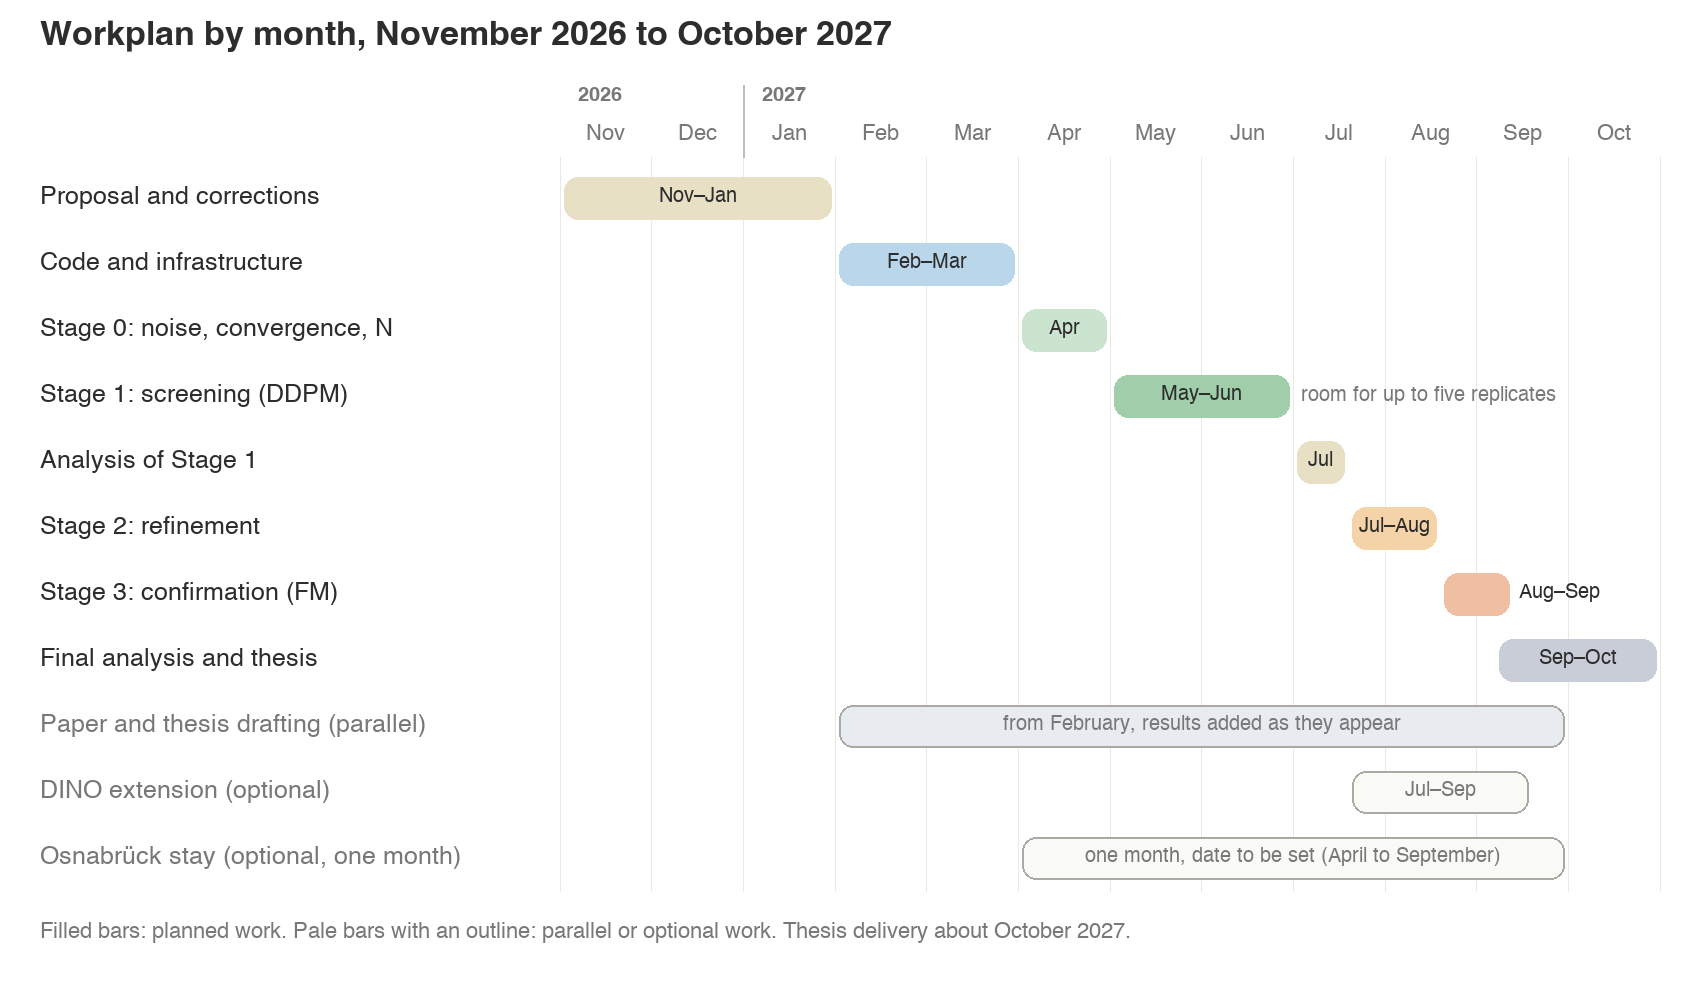
\includegraphics[width=0.95\textwidth]{Imagenes/gantt_workplan.png}
\caption{Workplan by calendar month. Filled bars are planned work; pale bars with an outline are parallel or optional work.}
\label{fig:gantt}
\end{figure}

The research phase lasts about eight months, from February to October 2027. The main risks are the availability of the cluster, which limits the work to four jobs at a time, the storage quota, and runs that fail or diverge. Stage 1 is scheduled for May and June because its runs need little attention; if the standard deviation measured in Stage 0 is larger than expected, the number of replicates is increased up to five, which that period allows, and, if more were needed, the schedule would be extended.
